Das Upload-System von LearnHub wurde so gestaltet, dass PDF-Dateien 
zusammen mit allen nötigen Metadaten in einem einzigen Request 
ans Backend geschickt werden können. Gleichzeitig musste eine 
Lösung gefunden werden um Schüler:innen von Lehrkräften zu 
unterscheiden, ohne ein eigenes Rollenmanagement von Grund auf 
zu bauen.

\subsection{Multipart File Upload}

Beim Hochladen einer Mitschrift muss das Frontend gleichzeitig 
zwei verschiedene Arten von Daten ans Backend schicken: eine 
PDF-Datei und mehrere Textfelder wie Titel, Beschreibung und 
die E-Mail-Adresse der zuständigen Lehrkraft. Dafür wird das 
\textbf{Multipart/Form-Data} Format verwendet, das seit 1998 
als Internetstandard (RFC 2388) für Datei-Uploads in 
Webanwendungen eingesetzt wird \cite{rfc2388}.

Das Grundprinzip ist einfach: Alle Informationen, also sowohl 
der Text als auch die Datei, werden gemeinsam in einem einzigen 
HTTP-Request ans Backend geschickt, ähnlich wie ein Brief mit 
Anhang.

Im Angular-Frontend wird dafür das eingebaute Browser-Objekt 
\texttt{FormData} verwendet, das keine zusätzlichen Bibliotheken 
braucht \cite{mdn_formdata}. Wie in 
Abbildung~\ref{fig:upload-formdata} zu sehen, werden die 
PDF-Datei sowie alle Metadaten wie Titel, Beschreibung, 
Uploadername und Lehrer-E-Mail einzeln ans 
\texttt{FormData}-Objekt angehängt und gemeinsam ans Backend 
gesendet.

\begin{figure}[H]
    \centering
    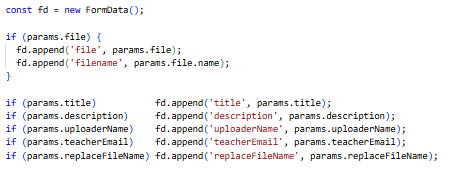
\includegraphics[width=0.85\textwidth]{pics/upload_formdata.png}
    \caption{FormData Implementierung im Frontend}
    \label{fig:upload-formdata}
\end{figure}

Im Quarkus-Backend wird der Multipart-Request über die 
\texttt{RESTEasy} Bibliothek verarbeitet, die automatisch mit 
Quarkus mitgeliefert wird \cite{quarkus_multipart}. Der 
Endpoint ist mit \texttt{@POST}, \texttt{@Path("/upload")} und 
\texttt{@Consumes(MediaType.MULTIPART\_FORM\_DATA)} annotiert.

\begin{figure}[H]
    \centering
    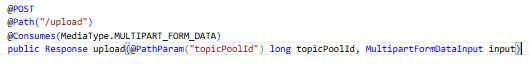
\includegraphics[width=0.85\textwidth]{pics/upload_endpoint.png}
    \caption{Quarkus Upload Endpoint}
    \label{fig:upload-endpoint}
\end{figure}

Multipart wurde bewusst gegenüber Base64-Kodierung gewählt. 
Bei Base64 würde die PDF-Datei erst in einen langen Text 
umgewandelt und als JSON übertragen werden, was die Dateigröße 
um ca. 33\% erhöht und zusätzlichen Rechenaufwand verursacht 
\cite{rfc2388}. Multipart schickt die Datei direkt als 
Binärdaten, was effizienter und schneller ist.

\subsection{Speicherung mit meta.json}

Nachdem die PDF erfolgreich gespeichert wurde, legt das Backend 
automatisch eine \textbf{meta.json} Datei an. Diese enthält 
alle relevanten Infos zur Mitschrift: Titel, Name des Uploaders, 
die Keycloak-ID der hochladenden Person (\texttt{uploaderSub}), 
die E-Mail der zuständigen Lehrkraft (\texttt{teacherEmail}), 
deren Keycloak-ID (\texttt{teacherSub}), den Zeitstempel und 
den aktuellen Freigabestatus.

Abbildung~\ref{fig:upload-meta} zeigt die auf dem Server 
gespeicherten meta.json Dateien, organisiert nach Themenpool-ID. 
Jede PDF hat eine gleichnamige meta.json im selben Ordner.

\begin{figure}[H]
    \centering
    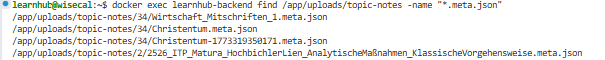
\includegraphics[width=0.85\textwidth]{pics/upload_meta.png}
    \caption{Auf dem Server gespeicherte meta.json Dateien}
    \label{fig:upload-meta}
\end{figure}

Besonders wichtig sind \texttt{uploaderSub} und 
\texttt{teacherSub}, also die eindeutigen Keycloak-IDs der 
beteiligten Personen. Diese IDs sind der zentrale 
Identifikationsmechanismus im gesamten Freigabeprozess 
\cite{ionos_docker}.

Der Vorteil dieser Trennung von Inhalt und Metadaten: Der 
Status einer Mitschrift kann jederzeit durch eine einfache 
Änderung in der meta.json aktualisiert werden, ohne die 
PDF-Datei selbst anfassen zu müssen.

\subsection{Warum kein CDN und keine Datenbank für PDFs}

Bei der Konzeption des Upload-Systems wurden zwei Alternativen 
bewusst verworfen.

Ein \textbf{Content Delivery Network} wie AWS S3 oder Google 
Cloud Storage hätte eine schnellere Auslieferung ermöglicht, 
wäre aber mit laufenden Kosten verbunden. Außerdem wäre eine 
externe Cloud-Abhängigkeit datenschutzrechtlich problematisch, 
da die Mitschriften der Schüler:innen auf Servern eines 
amerikanischen Unternehmens gespeichert würden. Durch die 
lokale Speicherung auf dem HTL-Server bleiben alle Daten im 
Einflussbereich der Schule \cite{redhat_container}.

Die Speicherung der PDFs direkt in MySQL als \texttt{BLOB} 
wurde ebenfalls verworfen. Datenbanken sind für strukturierte 
Daten wie Texte und Zahlen optimiert, nicht für große 
Binärdateien \cite{docker_overview}. Die direkte 
Dateisystem-Speicherung ist hier performanter und einfacher 
zu verwalten.

\subsection{Rollenerkennung über den distinguishedName}

Da LearnHub Keycloak zur Authentifizierung verwendet, der 
wiederum mit dem LDAP-Verzeichnis der HTL verbunden ist, 
enthält der JWT-Token auch LDAP-spezifische Felder wie den 
\textbf{distinguishedName}, der die Position der Person 
im Schulnetzwerk beschreibt \cite{ionos_docker}. Wie in 
Abbildung~\ref{fig:upload-dn-read} zu sehen, wird dieser 
Wert über \texttt{jwt.getClaim()} direkt aus dem Token 
ausgelesen.

\begin{figure}[H]
    \centering
    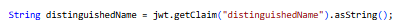
\includegraphics[width=0.85\textwidth]{pics/upload_dn_read.png}
    \caption{Auslesen des distinguishedName aus dem JWT-Token}
    \label{fig:upload-dn-read}
\end{figure}

Dann wird geprüft ob \texttt{OU=STUDENTS} im DN enthalten ist. 
Wenn ja, ist die Person eine Schüler:in, sonst eine Lehrkraft. 
Als Fallback wird zusätzlich geprüft ob die E-Mail-Adresse auf 
\texttt{@students.htl-leonding.ac.at} endet \cite{ionos_docker}. 

\begin{figure}[H]
    \centering
    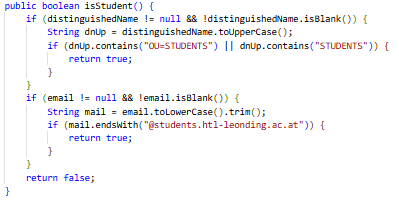
\includegraphics[width=0.85\textwidth]{pics/upload_dn_check.png}
    \caption{Rollenerkennung über den distinguishedName}
    \label{fig:upload-dn-check}
\end{figure}

\subsection{Lehrerliste im Arbeitsspeicher}

Für das Dropdown zur Auswahl der Lehrkraft beim Upload wird 
eine vollständige Liste aller Lehrkräfte der HTL benötigt. 
Diese Liste ist direkt im Backend als statische Liste 
hinterlegt und wird beim Start der App einmalig in den 
Arbeitsspeicher geladen und als \texttt{ConcurrentHashMap} 
gehalten.

Der Grund: Lehrkräfte registrieren sich nicht aktiv bei 
LearnHub. Eine Schüler:in muss aber schon beim Upload eine 
Lehrkraft auswählen können, bevor sich diese jemals eingeloggt 
hat. Würde die Liste nur aus der Datenbank geladen, wäre sie 
am Anfang leer. Wenn sich eine Lehrkraft zum ersten Mal 
einloggt, wird ihr Keycloak-Sub automatisch mit dem 
vorhandenen Datensatz verknüpft.